% Metódy inžinierskej práce

\documentclass[10pt,twoside,slovak,a4paper]{article}

\usepackage[slovak]{babel}
%\usepackage[T1]{fontenc}
\usepackage[IL2]{fontenc} % lepšia sadzba písmena Ľ než v T1
\usepackage[utf8]{inputenc}
\usepackage{graphicx}
\usepackage{url} % príkaz \url na formátovanie URL
\usepackage{hyperref} % odkazy v texte budú aktívne (pri niektorých triedach dokumentov spôsobuje posun textu)
\usepackage{cite}
%\usepackage{times}
\usepackage[nomarginpar, margin=1.6in]{geometry}%margin inconsistency


\pagestyle{headings}

\title{Agilné postupy pri vývoji medicínskeho softvéru\thanks{Semestrálny projekt v predmete Metódy inžinierskej práce, ak. rok 2021/22, vedenie: Ing. Vladimír Mlynarovič PhD.}} 

\author{Irina Makarova\\[2pt]
	{\small Slovenská technická univerzita v Bratislave}\\
	{\small Fakulta informatiky a informačných technológií}\\
	{\small \texttt{xmakarovai@stuba.sk}}
	}

%\date{\small 4. oktober 2021}



\begin{document}
%\renewcommand{\abstractname}{\vspace{-\baselineskip}} %removes abstract heading
\maketitle

\begin{abstract}
V súčasnosti sa rýchlo vyvíja trh zdravotníckych prenositeľných zariadení. Vodopádový model, ktorý sa klasicky používal pri vývoji bezpečnostne kritického softvéru, už pre svoju zdĺhavosť a nepružnosť nepredstavuje optimálny postup. Do popredia sa dostávajú rôzne agilné a kombinované prístupy, čo prináša so sebou otázku, ako implementovať do procesu vývoja agilné metódy a pri tom dodržať požadované normy. Tento článok prináša stručný prehľad aktuálne platných noriem; vysvetľuje podstatu vodopádového a agilných modelov (Scrum, XP, DSDM), porovnáva ich a poukazuje na črty jednotlivých stratégií, ktoré sú prínosné pre túto oblasť. V článku sa uvádzajú niektoré existujúce riešenia, ako sa tieto modely dajú efektívne kombinovať pri vývoji medicínskeho softvéru.
\end{abstract}

\section{Úvod} 
Digitalizácia prebieha vo všetkých sférach spoločenského života. Aj oblasť zdravotníctva čoraz viac spolieha na zariadenia so vstavaným softvérom, vzrastá dopyt po mobilných aplikáciách slúžiacich na monitorovanie, predikciu alebo korekciu zdravotných problémov. Vývoj medicínskeho softvéru má prebiehať v súlade s platnými normami. Požiadavky uvedené v normách a smerniciach sú všeobecné a nemožno ich jednoducho nasadiť do praxe. Klasický sekvenčný prístup zdanlivo najlepšie pokrýva všetky rozmanité požiadavky. Tento postup má však jednu zásadnú nevýhodu – netoleruje zmeny. V rýchlo sa meniacom svete technológií na každom stupni vývoja môže nastať potreba niečo upraviť s ohľadom na nové požiadavky. Okrem toho sa produkt musí rýchlo dostať k užívateľom, aby mal šancu etablovať sa na trhu\cite{mchugh2013}. 

Agile si osvojili softvérové spoločnosti po celom svete. 84\% respondentov pracujúcich v oblasti softvérového inžinierstva uviedlo, že ich tím využíva nejakú formu agile. Hlavnými príčinami popularity týchto metodík je ich efektívnosť, flexibilnosť a urýchlené dodanie funkčného produktu\cite{agileReport}. Ešte pred pár rokmi ich miera adopcie v doméne vývoja bezpečnostne kritických systémov, akým je aj medicínsky softvér, bola nízka. Jedným z dôvodov bolo to, že agilné postupy sa javia byť v rozpore s regulačnými požiadavkami. Výrobcovia softvéru pre medicínske zariadenia sú pre schválenie produktu povinní predkladať rozsiahlu dokumentáciu, avšak jeden z agilných princípov znie “Funkčný softvér je viac ako vyčerpávajúca dokumentácia“\cite{mchugh2013}. Aj keď samostatne žiadna z agilných metodík naozaj nie vhodná na vývoj zdravotníckeho softvéru, zavedením vybraných agilných praktík sa proces vývoja dá zoptimalizovať a lepšie prispôsobiť aktuálnemu stavu prostredia\cite{mccaffery2019}. A preto sa v súčasnosti veľa firiem vyvíjajúcich zdravotnícky softvér riadi hybridnými modelmi\cite{hybridReport}. Tvorba a validácia takéhoto modelu je náročná a zdĺhavá. Existuje ale niekoľko riešení vytvorených pre oblasť zdravotníctva. V tomto článku budú podrobnejšie predstavené dva z nich – rámec MDevSPICE a agilný V-model. Hlavným cieľom daného článku je poukázať na užitočnosť agilných prístupov vo vývoji zdravotníckeho softvéru a vysvetliť na príkladoch ako sa klasické a iteratívne modely dajú výhodne kombinovať tak, aby sa vzájomne dopĺňali. 


\section{Normy pre medicínsky softvér}
Podľa nariadenia o zdravotníckych pomôckach 2017/745 (MDR) sa za zdravotnícku pomôcku považuje akýkoľvek výrobok, ktorý je výrobcom určený na použitie za účelmi ako sú diagnostika, predikcia, sledovanie, prevencia, liečba alebo zmiernenie choroby, a ktorý nedosahuje svoj účinok pomocou farmakologických alebo imunologických prostriedkov. Pod túto definíciu spadá nielen softvér zabudovaný v špecializovaných prístrojoch ale aj softvér ako taký, tzv. SaMD (Software as a Medical Device). Zdravotnícky softvér sa zaraďuje medzi bezpečnostne kritický softvér. To znamená, že jeho nesprávna funkčnosť môže ohroziť zdravie, alebo dokonca život človeka. V závislosti od rizík spojených s jeho používaním sa softvér klasifikuje na tri triedy. Z tejto klasifikácie potom vyplývajú spôsoby, akými sa preukazuje jeho bezpečnosť, a požiadavky, ktoré má spĺňať. V závislosti od regiónu, v ktorom sa má zdravotnícka pomôcka uviesť na trh, sa musia dodržiavať rôzne normy alebo usmernenia. V USA je to Úrad pre kontrolu potravín a liečiv (FDA). Vo všeobecnosti platí, že pri posudzovaní a schvaľovaní zdravotníckych pomôcok v Európskej únii neexistuje žiadny centralizovaný regulačný orgán, ako napríklad Európska agentúra pre lieky (EMA), alebo americký úrad FDA. V EÚ výrobca musí preukázať, že produkt spĺňa platné štandardy. Kľúčovým štandardom pre vývojárov medicínskeho softvéru je ISO IEC 62304:2006. Podľa neho musí vývoj softvéru prebiehať podľa vopred stanoveného modelu životného cyklu, jeho výber je však na výrobcovi\cite{bronneke2021}.

\section{Modely riadenia vývoja softvéru}
Všeobecne sa proces vývoja softvéru dá organizovať dvoma spôsobmi – sekvenčne a iteratívne. Pri tradičnom prístupe sa najprv zostavuje dokument všetkých požiadaviek na softvérový produkt. A na základe neho sa potom navrhuje a implementuje produkt. Môže sa však stať, že požiadavky, ktoré zadá zákazník budú nepresné a neúplné, alebo sa pri testovaní v neskorších fázach objaví chyba. Vtedy sa bude treba vracať k predchádzajúcim etapám vývoja softvéru a aplikovať nové požiadavky na návrh, testovanie alebo implementáciu. V dôsledku častých alebo výrazných zmien požiadaviek je potom nutné zvýšiť rozpočet alebo oddialiť termín dodania. Toto zase môže viesť až k nepoužiteľnosti vytvorených softvérových systémov kvôli ich neaktuálnosti\cite{AVmodelPrax}. Snaha nájsť alternatívu tomuto postupu vyústila k vzniku množstva techník a rámcov, ktoré sa všeobecne volajú agile. Základné princípy agile boli sformulované skupinou 17 vývojárov v roku 2001 a sú zadokumentované v Manifeste pre agilný vývoj softvéru, ktorý postuluje nasledujúce\cite{agileManifesto}: 
\begin{itemize}
\item Ľudia a komunikácia sú viac ako len procesy a nástroje
\item Funkčný softvér je viac ako vyčerpávajúca dokumentácia
\item Spolupráca so zákazníkom je viac ako dojednávanie zmluvy
\item Radšej reagovať na zmenu ako sa držať plánu
\end{itemize}
Dodržiavať tieto hodnoty v praxi umožňuje inkrementálny spôsob vývoja a tesná spolupráca so zákazníkom. Agilné metodiky sú iteratívne – tvorba projektu prebieha v cykloch. Každý cyklus, alebo iterácia, sa dá chápať ako menší projekt, ktorého výstupom je vždy funkčná otestovaná verzia produktu. Výsledkom toho je, že sa k zákazníkovi už po prvých iteráciách dostane prevádzková verzia softvéru, ktorú vie vyskúšať a poskytnúť spätnú väzbu. Prípadné pripomienky zákazníka sa potom stávajú súčasťou nasledujúcej iterácie. Táto prispôsobivosť zmenám a flexibilita požiadaviek má významný dopad na kvalitu produktu a jeho prijatie zákazníkom. 

\textbf{V-model} je v oblasti vývoja zdravotníckeho softvéru najpoužívanejším modelom. Je rozšírením vodopádového modelu. Dáva do súvislosti v ňom špecifikované vývojové aktivity s testovacími aktivitami. Pozostáva z dvoch vetiev, ktoré znázorňujú časovú postupnosť jednotlivých etáp vývoja a testovania\cite{mchugh2013}.

\textbf{Scrum} je predovšetkým spôsob manažmentu, menej sa zaoberá technickou stránkou softvérového inžinierstva. V súčasnosti je najrozšírenejším agilným rámcom\cite{agileReport}. Vývoj podľa scrum predstavuje postupnosť pevne časovo ohraničených cyklov, tzv. sprintov. Po skončení každého z nich má tím byť schopný dodať potenciálne nasaditeľný produkt. Kontrola a prispôsobenie procesu vývoja sa vykonáva počas denných porád a taktiež na konci každého sprintu. Aktivita na projekte sa priebežne zaznamenáva v štyroch hlavných dokumentoch – produktový backlog (zoznam požiadaviek na produkt), sprint backlog (zoznam úloh pre daný sprint), release burndown (sledovanie ešte nerealizovaných položiek produktového backlogu), sprint burndown (sledovanie ešte nerealizovaných položiek v rámci prebiehajúceho sprintu)\cite{scrum}.

\textbf{Extrémne programovanie (XP)} je agilný rámec, ktorý zhrňuje praktiky softvérového inžinierstva tak, aby sa dalo vyvíjať čo najkvalitnejší produkt v udržateľnom čase. Najdôležitejšími z týchto praktík sú: jednoduchý návrh, refaktorizácia, priebežné testovanie funkčných blokov, programovanie v pároch, krátke iterácie, tesná prepojenosť so zákazníkom, použitie metáfor pre zjednodušenie komunikácie so zákazníkom\cite{XP}.

\textbf{Metóda dynamického vývoja systémov} definuje postupy a pravidlá pre každé štádium životného cyklu vývoja softvéru. Ideový základ DSDM tvorí osem princípov - sústredeďte sa na potreby zákazníka, dodávajte načas, spolurácujte, prvoradá je kvalita, vyvíjajte interatívne a inkrementálne vychádazjúc z pevných základov, komunikujte jasne a kontinuálne, buďte schopní kedykoľvek preukázať, že projekt je pod kontrolou. DSDM sa menej zaoberá programovacimi prístupmi, ale podporuje skôr riadenie projektov. Dá sa kombinovať s inými agilnými metodikami\cite{dsdm}.

\section{Kombinované prístupy}
Prieskumy naznačujú, že hlavným cieľom pri kombinovaní rôznych prístupov je dodržanie rozmanitých požiadaviek kladených regulačnými orgánmi. Pre mnohých respondentov je kombinovanie praktík zo sekvenčných a iteratívnych modelov náročné, a súčasný kombinovaný model vytvorili pomocou metódy pokusu a omylu\cite{hybridReport}. Z toho vyplýva, že v sfére vývoja bezpečnostne kritického softvéru stále je nedostatok overených hybridných modelov, taktiež je možné, že informovanosť firiem o ich existencii je nízka. Nižšie sú popísané dva nádejné modely navrhnuté špeciálne pre vývoj zdravotníckeho softvéru.

\textbf{MDevSPICE} bol vytvorený s cieľom zhrnúť obsah noriem pre vývoj zdravotníckeho softvéru do jedného rámca, ktorý poskytne spoločnostiam prehľad o základných požiadavkách a taktiež umožní zistiť silné a slabé stránky postupu, ktoré aktuálne používajú. Rámec pozostáva z procesného referenčného modelu (PRM), ktorý obsahuje normatívne požiadavky, a modelu posúdenia procesu (MPP), ktorý umožňuje zhodnotiť praktiky podľa toho, či zodpovedajú požiadavkám popísaným v PRM. PRM predstavuje štruktúrovaný súbor procesov, ich cieľov a výsledkov. Výsledkami procesu sú normatívne požiadavky, ktoré proces má spĺňať, aby dosiahol svoj účel. Kostru PRM tvorí norma IEC 62304, ktorá stanovuje všeobecné požiadavky na životný cyklus vývoja zdravotníckeho softvéru. PRM pozostáva z 23 procesov, z ktorých 10 sa týkajú systému ako celku, 8 – softvéru a zvyšných 5 podporuje ako životný cyklus softvéru, tak aj systému, ktorého súčasťou ten softvér je. MPP pozostáva z dvoch častí – dimenzia procesu a dimenzia kvality. Atribútmi každého procesu sú jeho názov, účel, výsledky, aktivity, pracovné produkty a ich charakteristiky. Dimenzia kvality bola odvodená priamo z normy ISO/IEC 15504-5 prezývanej tiež SPICE a slúži na vyhodnotenie kvality procesov v danom softvérovom projekte\cite{ramecmd}.

\begin{center}
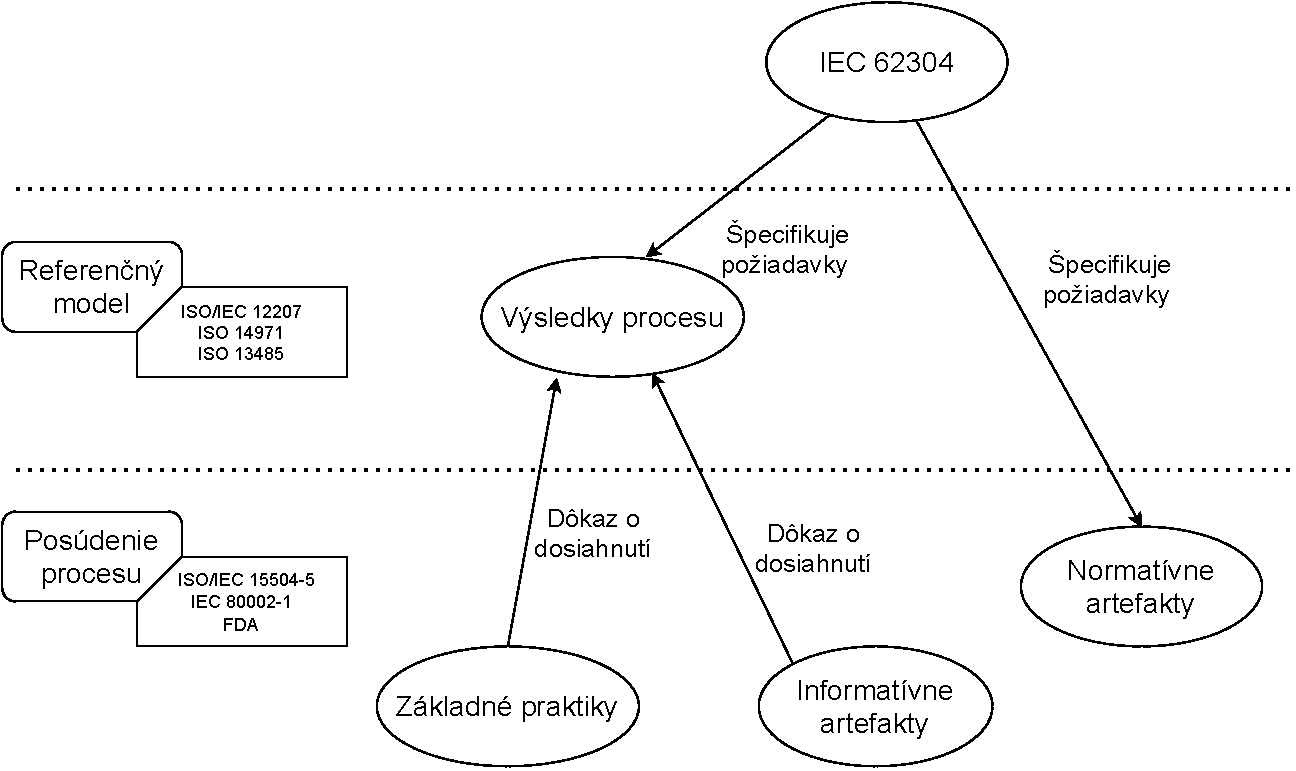
\includegraphics[scale=0.5]{MDevSPICE.pdf}
\end{center}
\textbf{Obrázok 1.} Základné prvky rámca MDevSPICE - procesný referenčný model a model posudzovania procesu. Upravené podľa\cite{ramecmd}.
\medskip

MDevSPICE prešiel medzinárodnými expertnými skúškami a bol otestovaný v praxi viacerými spoločnosťami. Špeciálne pre vývoj medicínskych mobilných aplikácií bol na základe tohto rámca vytvorený rámec MMA. Vývoj softvéru, ktorý je súčasťou mobilných zariadení má svoje špecifiká. Napríklad, krátkosť času vstupu na trh je tu obzvlášť dôležitá, zabezpečenie sledovateľnosti je náročné, neľahké je aj použitie vo finálnom produkte softvéru vyvinutého treťou stranou (tzv. SOUP). Všetky tieto otázky sú v MMA zohľadnené\cite{mobileMed}.

V súvislosti s narastajúcou popularitou hybridných a agilných prístupov v danej oblasti bolo autormi urobené detailné porovnanie rámca MDevSPICE s agilnými rámcami Scrum, XP a metodikou DSDM. Výsledky analýzy sú zhrnuté v tabuľke 1. Mapovanie procesov XP odhalilo nedostatočnú podporu manažmentu, čo sa dalo doplniť kombinovaním so Scrum. Spolu tieto rámce pokryli 9 z 23 procesov v modeli MDevSPICE. Metodika DSDM poskytla čiastočné alebo úplne pokrytie 13 procesov. Pokrytie pre daný proces sa počítalo ako pomer počtu aktivít definovaných v analyzovanom rámci a počtu aktivít podľa rámca MDevSPICE\cite{mccaffery2019}. 
\medskip

\noindent\textbf{Tabuľka 1.} Porovnanie rámcov XP, DSDM a Scrum podľa počtu spoločných procesov s rámcom MDevSPICE.
\begin{table}[h!]
\centering
\begin{tabular}{l|c|c|c|}
 & XP & DSDM & Scrum \\
Úplne pokrytých procesov     & 0  & 3    & 1 \\
Čiastočne pokrytých procesov & 7  & 10   & 4 \\
\end{tabular}
\end{table}
\medskip

\textbf{Agilný V-model} ako je vidieť z obrázku 2 rozširuje klasický V-model o agilné praktiky, je jeho nadstavbou. V-model bol autormi zvolený ako základ práve preto, že mnohé firmy ho už dobre poznajú a majú s ním dlhoročné skúsenosti. Na prechod do hybridného procesu vývoja je potrebná nielen znalosť agilných techník, ale aj istá miera odvahy. Tento model zmierňuje obidve prekážky. Jednak vymenúva konkrétne agilné praktiky, ktoré sú použiteľné a mapuje ich na jednotlivé fázy V-modelu. A na druhej strane využitie známeho V-modelu ako základu eliminuje strach z nového a neistotu tímov\cite{mchugh2013}.

\begin{center}
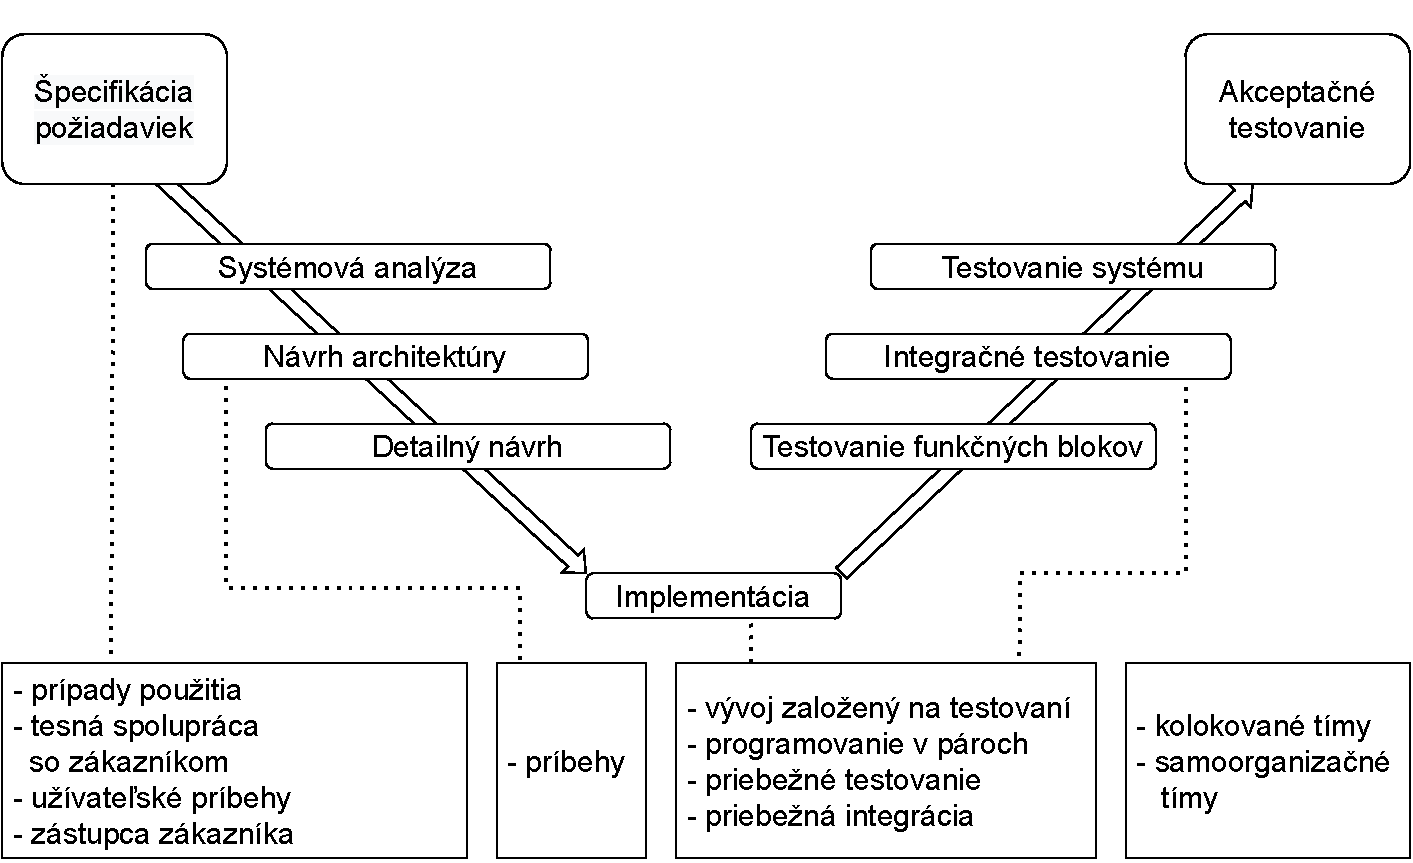
\includegraphics[scale=0.5]{avmodel.pdf}
\end{center}
\textbf{Obrázok 2.} Agilný V-model. Plné čiary znázorňujú prechod medzi fázami vývoja. Prerušované čiary spájajú agilné metodiky s fázami, do ktorých môžu byť inkorporované. Dve praktiky nie sú spojené so žiadnou fázou, lebo sa týkajú organizácie tímov a nie procesu. Upravené podľa\cite{mchugh2013}.
\medskip

Tvorba tohto modelu prebiehala v spolupráci mnohými organizáciami. Daný model sa aj vyskúšal vo firme BBT, ktorá sa predtým riadila V-modelom a pri práci sa vo veľkej miere spoliehala na dopredné plánovanie. A preto zapracovanie zmien do vyvíjaného produktu bolo identifikované ako hlavný problém. V snahe zmieniť tento problém firma zaviedla inkubačnú dobu, ktorá predchádzala vývoju a dávala všetkým zainteresovaným stranám čas na odhalenie nepresností v požiadavkách. S ohľadom tieto skutočnosti bol autormi navrhnutý agilný V-model, ktorý prevzal niektoré praktiky z rámca Scrum a metodiky XP. Iteratívny prístup spočíval v tom, že sa výsledný softvérový produkt rozdelil na komponenty, a tie – na ešte menšie prvky, a jednotlivé prvky sa vytvárali v nezávislých cykloch. K integrovaniu komponentov dochádzalo v neskorších štádiách, pričom žiadna z požiadaviek sa nepovažovala za splnenú, kým každý komponent neprešiel fázu implementácie. Z rámca Scrum boli prebrané dokumenty umožňujúce sledovať stav projektu, ohraničenie času (time-boxing), technika odhadu Scrum poker, roly, denné porady, aktivity ohľadom plánovania šprintov. Z extrémneho programovania to boli refaktorizácia a vývoj riadený testovaním. Tento na mieru vytrovený AV-model sa následne vyskúšal v praxi na jednom projekte. AV-model zefektívnil proces vývoja a komunikácie so zákazníkom. Na záverečných pohovoroch členovia tímu urobili odhad, že projekt by sa predĺžil o 14\% a rozpočet prekročil o 7\%, keby postupovali podľa V-modelu\cite{AVmodelPrax}.

\section{Vyjadrenie k témam z prednášok}
\paragraph{Technológie a ľudia} 
Ľudia a technológie sa vzájomne ovplyvňujú. Zmeny v spoločnosti vedú k vzniku nových technológií a rozvoj technológií zase mení ľudí, ktorí ich používajú aj vytvárajú. Tak napríklad, agilné metodiky vývoja softvéru vznikli ako odpoveď na rýchly rozvoj technológií. Výhodu dostávali tie firmy, ktoré prišli na trh s inovatívnym riešením ako prvé; rástla konkurencia. Vznikla potreba dodávať kvalitné produkty v relatívne krátkom čase. Agilné metodiky a rámce priniesli ďalšiu výhodu oproti tradičným prístupom – umožnili prispôsobovať proces vývoja meniacim sa požiadavkám. Agilné projektové riadenie je orientované na ľudí. Kým tradičné prístupy sa snažia riešeniu ľudského faktora vyhnúť, agile vyžaduje tesnú spoluprácu medzi všetkými členmi tímu a zainteresovanými stranami, víta zmeny a vie sa vysporiadať s prípadnými chybami pri ich neskoršom odhalení.
\paragraph{Udržateľnosť a etika}
Pre hodnotenie procesu z pohľadu udržateľnosti je užitočná SWOT analýza, ktorá slúži na identifikáciu vnútorných a vonkajších faktorov, ktoré prospievajú a bránia dosiahnutiu cieľa. Pričom silné a slabé stránky sú vnútorné atribúty; príležitosti a ohrozenia – externé podmienky. Náčrt takejto analýzy predstavím na príklade kombinovaných modelov vývoja softvéru. Silné stránky – proces vývoja sa dá prispôsobiť meniacim sa požiadavkám; priebežné testovanie umožňuje odhaliť chyby skôr; dokumentácia nie je zasiahnutá ako pri rýdzo agilných rámcoch a metodikách. Slabé stránky – zo strany zákazníka sa očakáva silná zainteresovanosť do procesu; obmedzené množstvo osvedčených hybridných modelov v istých doménach (napr. v zdravotníctve). Príležitosti – vyššia miera motivovanosti členov vývojárskeho tímu, lebo spolu s agilnými praktikami sa zavádzajú aj agilné hodnoty (tímová práca, každý názor je dôležitý, tím samostatne určuje najlepšiu cestu atď.). Ohrozenia – v tímoch, ktoré sa dlhodobo riadili sekvenčnými modelmi, je integrácia sťažená; nesprávna interpretácia agilných praktík a hodnôt.

\section{Záver}
Mnohé firmy si osvojili agilné praktiky kvôli ich flexibilite. Zvyčajne sa agile používa v kombinácii s tradičnými praktikami. V oblasti vývoja medicínskeho softvéru problémom je nedostatok overených hybridných modelov. Pri viacerých praktikách a modeloch sa predpokladá, že by mohli byť pre túto oblasť prínosné, ale chýba ich otestovanie v praxi.
%Agilný V-model\cite{mchugh2013}
%Agilný V-model

% generuje zoznam literatúry z obsahu súboru literatura.bib
\bibliography{literatura}
\bibliographystyle{plain} % alpha/ abbrv/ plain
\end{document}
